% Options for packages loaded elsewhere
\PassOptionsToPackage{unicode}{hyperref}
\PassOptionsToPackage{hyphens}{url}
%
\documentclass[
  ignorenonframetext,
]{beamer}
\usepackage{pgfpages}
\setbeamertemplate{caption}[numbered]
\setbeamertemplate{caption label separator}{: }
\setbeamercolor{caption name}{fg=normal text.fg}
\beamertemplatenavigationsymbolsempty
% Prevent slide breaks in the middle of a paragraph
\widowpenalties 1 10000
\raggedbottom
\setbeamertemplate{part page}{
  \centering
  \begin{beamercolorbox}[sep=16pt,center]{part title}
    \usebeamerfont{part title}\insertpart\par
  \end{beamercolorbox}
}
\setbeamertemplate{section page}{
  \centering
  \begin{beamercolorbox}[sep=12pt,center]{part title}
    \usebeamerfont{section title}\insertsection\par
  \end{beamercolorbox}
}
\setbeamertemplate{subsection page}{
  \centering
  \begin{beamercolorbox}[sep=8pt,center]{part title}
    \usebeamerfont{subsection title}\insertsubsection\par
  \end{beamercolorbox}
}
\AtBeginPart{
  \frame{\partpage}
}
\AtBeginSection{
  \ifbibliography
  \else
    \frame{\sectionpage}
  \fi
}
\AtBeginSubsection{
  \frame{\subsectionpage}
}

\usepackage{amsmath,amssymb}
\usepackage{lmodern}
\usepackage{iftex}
\ifPDFTeX
  \usepackage[T1]{fontenc}
  \usepackage[utf8]{inputenc}
  \usepackage{textcomp} % provide euro and other symbols
\else % if luatex or xetex
  \usepackage{unicode-math}
  \defaultfontfeatures{Scale=MatchLowercase}
  \defaultfontfeatures[\rmfamily]{Ligatures=TeX,Scale=1}
\fi
% Use upquote if available, for straight quotes in verbatim environments
\IfFileExists{upquote.sty}{\usepackage{upquote}}{}
\IfFileExists{microtype.sty}{% use microtype if available
  \usepackage[]{microtype}
  \UseMicrotypeSet[protrusion]{basicmath} % disable protrusion for tt fonts
}{}
\makeatletter
\@ifundefined{KOMAClassName}{% if non-KOMA class
  \IfFileExists{parskip.sty}{%
    \usepackage{parskip}
  }{% else
    \setlength{\parindent}{0pt}
    \setlength{\parskip}{6pt plus 2pt minus 1pt}}
}{% if KOMA class
  \KOMAoptions{parskip=half}}
\makeatother
\usepackage{xcolor}
\newif\ifbibliography
\setlength{\emergencystretch}{3em} % prevent overfull lines
\setcounter{secnumdepth}{-\maxdimen} % remove section numbering


\providecommand{\tightlist}{%
  \setlength{\itemsep}{0pt}\setlength{\parskip}{0pt}}\usepackage{longtable,booktabs,array}
\usepackage{calc} % for calculating minipage widths
\usepackage{caption}
% Make caption package work with longtable
\makeatletter
\def\fnum@table{\tablename~\thetable}
\makeatother
\usepackage{graphicx}
\makeatletter
\def\maxwidth{\ifdim\Gin@nat@width>\linewidth\linewidth\else\Gin@nat@width\fi}
\def\maxheight{\ifdim\Gin@nat@height>\textheight\textheight\else\Gin@nat@height\fi}
\makeatother
% Scale images if necessary, so that they will not overflow the page
% margins by default, and it is still possible to overwrite the defaults
% using explicit options in \includegraphics[width, height, ...]{}
\setkeys{Gin}{width=\maxwidth,height=\maxheight,keepaspectratio}
% Set default figure placement to htbp
\makeatletter
\def\fps@figure{htbp}
\makeatother

\makeatletter
\@ifpackageloaded{tcolorbox}{}{\usepackage[many]{tcolorbox}}
\@ifpackageloaded{fontawesome5}{}{\usepackage{fontawesome5}}
\definecolor{quarto-callout-color}{HTML}{909090}
\definecolor{quarto-callout-note-color}{HTML}{0758E5}
\definecolor{quarto-callout-important-color}{HTML}{CC1914}
\definecolor{quarto-callout-warning-color}{HTML}{EB9113}
\definecolor{quarto-callout-tip-color}{HTML}{00A047}
\definecolor{quarto-callout-caution-color}{HTML}{FC5300}
\definecolor{quarto-callout-color-frame}{HTML}{acacac}
\definecolor{quarto-callout-note-color-frame}{HTML}{4582ec}
\definecolor{quarto-callout-important-color-frame}{HTML}{d9534f}
\definecolor{quarto-callout-warning-color-frame}{HTML}{f0ad4e}
\definecolor{quarto-callout-tip-color-frame}{HTML}{02b875}
\definecolor{quarto-callout-caution-color-frame}{HTML}{fd7e14}
\makeatother
\makeatletter
\makeatother
\makeatletter
\makeatother
\makeatletter
\@ifpackageloaded{caption}{}{\usepackage{caption}}
\AtBeginDocument{%
\ifdefined\contentsname
  \renewcommand*\contentsname{Table of contents}
\else
  \newcommand\contentsname{Table of contents}
\fi
\ifdefined\listfigurename
  \renewcommand*\listfigurename{List of Figures}
\else
  \newcommand\listfigurename{List of Figures}
\fi
\ifdefined\listtablename
  \renewcommand*\listtablename{List of Tables}
\else
  \newcommand\listtablename{List of Tables}
\fi
\ifdefined\figurename
  \renewcommand*\figurename{Figure}
\else
  \newcommand\figurename{Figure}
\fi
\ifdefined\tablename
  \renewcommand*\tablename{Table}
\else
  \newcommand\tablename{Table}
\fi
}
\@ifpackageloaded{float}{}{\usepackage{float}}
\floatstyle{ruled}
\@ifundefined{c@chapter}{\newfloat{codelisting}{h}{lop}}{\newfloat{codelisting}{h}{lop}[chapter]}
\floatname{codelisting}{Listing}
\newcommand*\listoflistings{\listof{codelisting}{List of Listings}}
\makeatother
\makeatletter
\@ifpackageloaded{caption}{}{\usepackage{caption}}
\@ifpackageloaded{subcaption}{}{\usepackage{subcaption}}
\makeatother
\makeatletter
\@ifpackageloaded{tcolorbox}{}{\usepackage[many]{tcolorbox}}
\makeatother
\makeatletter
\@ifundefined{shadecolor}{\definecolor{shadecolor}{rgb}{.97, .97, .97}}
\makeatother
\makeatletter
\makeatother
\ifLuaTeX
  \usepackage{selnolig}  % disable illegal ligatures
\fi
\IfFileExists{bookmark.sty}{\usepackage{bookmark}}{\usepackage{hyperref}}
\IfFileExists{xurl.sty}{\usepackage{xurl}}{} % add URL line breaks if available
\urlstyle{same} % disable monospaced font for URLs
\hypersetup{
  pdftitle={Section 1.1 Installation of R/RStudio},
  hidelinks,
  pdfcreator={LaTeX via pandoc}}

\title{Section 1.1 Installation of R/RStudio}
\author{}
\date{}

\begin{document}
\frame{\titlepage}
\ifdefined\Shaded\renewenvironment{Shaded}{\begin{tcolorbox}[borderline west={3pt}{0pt}{shadecolor}, enhanced, boxrule=0pt, sharp corners, frame hidden, breakable, interior hidden]}{\end{tcolorbox}}\fi

\begin{frame}
\end{frame}

\begin{frame}{What is R? What is RStudio?}
\protect\hypertarget{what-is-r-what-is-rstudio}{}
So far, we have been talking about something called ``R/RStudio''.
People familiar with this program know what this is about. However, it
can be quite confusing when we have never heard of it.

We are actually referring to two programs:

\begin{longtable}[]{@{}
  >{\centering\arraybackslash}p{(\columnwidth - 2\tabcolsep) * \real{0.5417}}
  >{\centering\arraybackslash}p{(\columnwidth - 2\tabcolsep) * \real{0.4583}}@{}}
\toprule()
\begin{minipage}[b]{\linewidth}\centering
R
\end{minipage} & \begin{minipage}[b]{\linewidth}\centering
RStudio
\end{minipage} \\
\midrule()
\endhead

\includegraphics[width=1.44792in,height=\textheight]{./assets/images/R_logo.png}
& 
\includegraphics{./assets/images/RStudio_Logo.png} \\
\bottomrule()
\end{longtable}

The main program is called R. This is where all the magic happens.
RStudio is a user-friendly interface such that it is easier to work
with.

Maybe a metaphor can help to understand the difference between R and
RStudio. As you are engaging yourself in this tutorial, I assume that
you have a computer (and that you are using one). You can create
folders, open Word or Excel documents, write in it and save them in the
folders you created.

\begin{tcolorbox}[enhanced jigsaw, colback=white, opacityback=0, bottomrule=.15mm, colframe=quarto-callout-tip-color-frame, rightrule=.15mm, left=2mm, colbacktitle=quarto-callout-tip-color!10!white, leftrule=.75mm, opacitybacktitle=0.6, bottomtitle=1mm, toprule=.15mm, coltitle=black, breakable, toptitle=1mm, titlerule=0mm, title=\textcolor{quarto-callout-tip-color}{\faLightbulb}\hspace{0.5em}{Think about it}, arc=.35mm]

Now it is time to reflect on what you are doing. You have done these
tasks by using your mouse or your touchpad and clicking on icons (or
figures) on your screen. What you may not know is that when doing so,
you have run many lines of codes. Actually, it is your computer that ran
them in programs able to perform computations. Your role has been to
trigger these programs by using the user-friendly interface installed in
your computer.

\end{tcolorbox}

This is the exact same thing with R and RStudio. R will perform the
computations that you ask for. And you will ask R to do stuff by
clicking on icons and writing commands using the user-friendly interface
of RStudio. And this is why you need to download two programs!

\begin{tcolorbox}[enhanced jigsaw, colback=white, opacityback=0, bottomrule=.15mm, colframe=quarto-callout-note-color-frame, rightrule=.15mm, left=2mm, colbacktitle=quarto-callout-note-color!10!white, leftrule=.75mm, opacitybacktitle=0.6, bottomtitle=1mm, toprule=.15mm, coltitle=black, breakable, toptitle=1mm, titlerule=0mm, title=\textcolor{quarto-callout-note-color}{\faInfo}\hspace{0.5em}{Anecdote}, arc=.35mm]

Let me share a personal anecdote when I just entered graduate school and
I had my very first class of language programming for linguistic
research. Just before leaving, the instructor said very quickly that we
had to, I quote, ``download R for next time''. I had never heard of R,
and to me, calling a program with only one letter seemed kind of
awkward. Therefore, I assumed that I misheard the instructions, or that
I missed some information. You can just imagine how surprised I was when
I googled ``R'' and actually found that this existed!

\end{tcolorbox}
\end{frame}

\begin{frame}{Download and install R and RStudio}
\protect\hypertarget{download-and-install-r-and-rstudio}{}
\begin{block}{Download and install R}
\protect\hypertarget{download-and-install-r}{}
You can download R for free from the official website
\href{https://www.r-project.org/}{here}.

You have to look for the link in the middle of the first paragraph on
the front page.

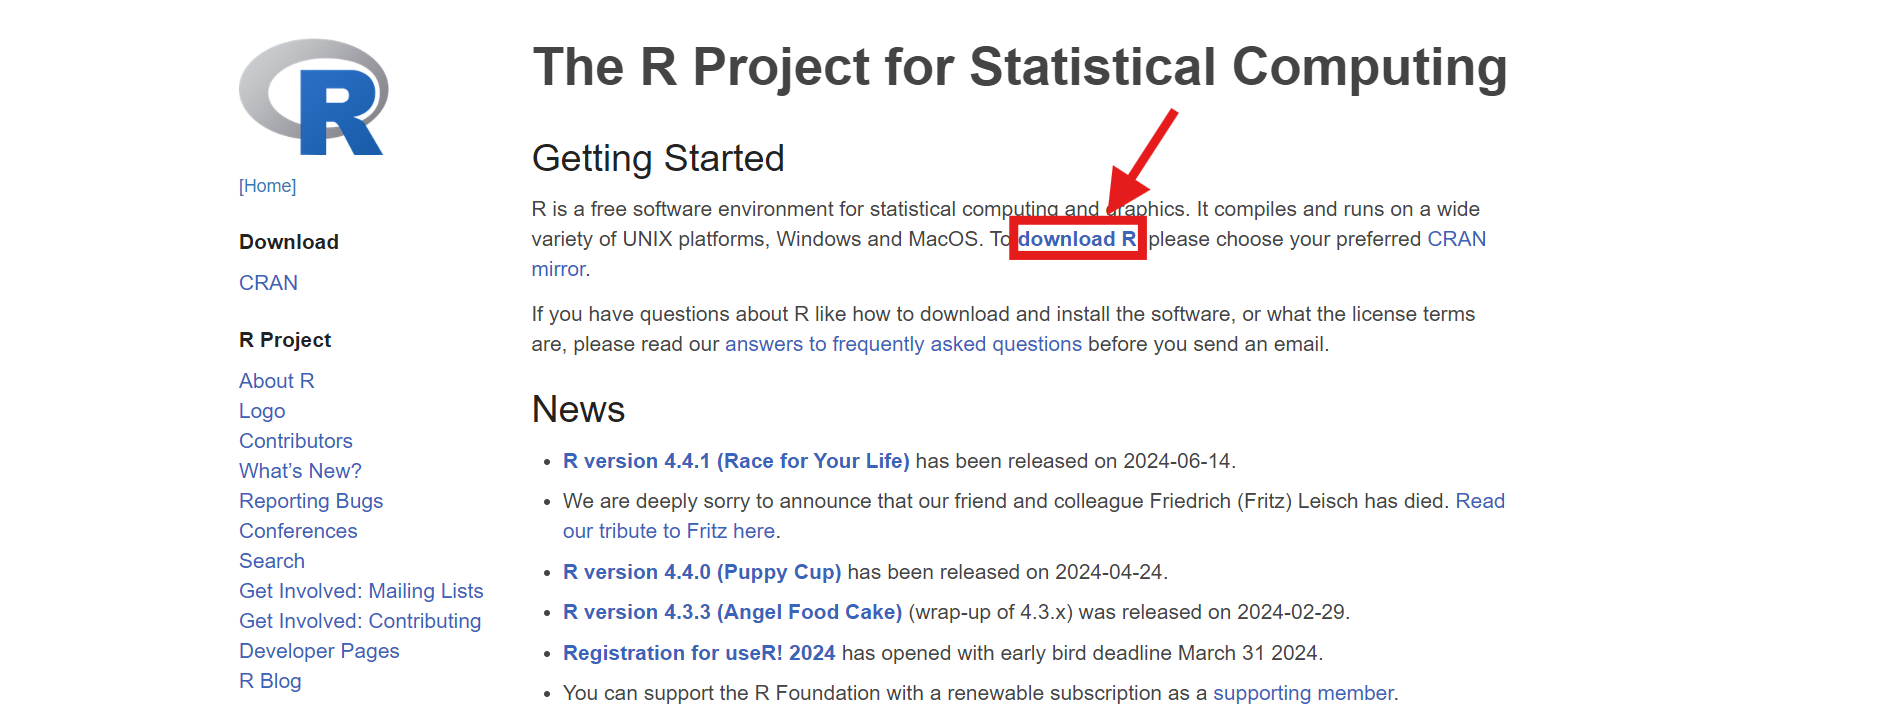
\includegraphics{./assets/images/RWebsite_FrontPage.png}

Then, you need to choose your CRAN. Let's choose the one in Taiwan. You
will need to scroll down the page to find the link.

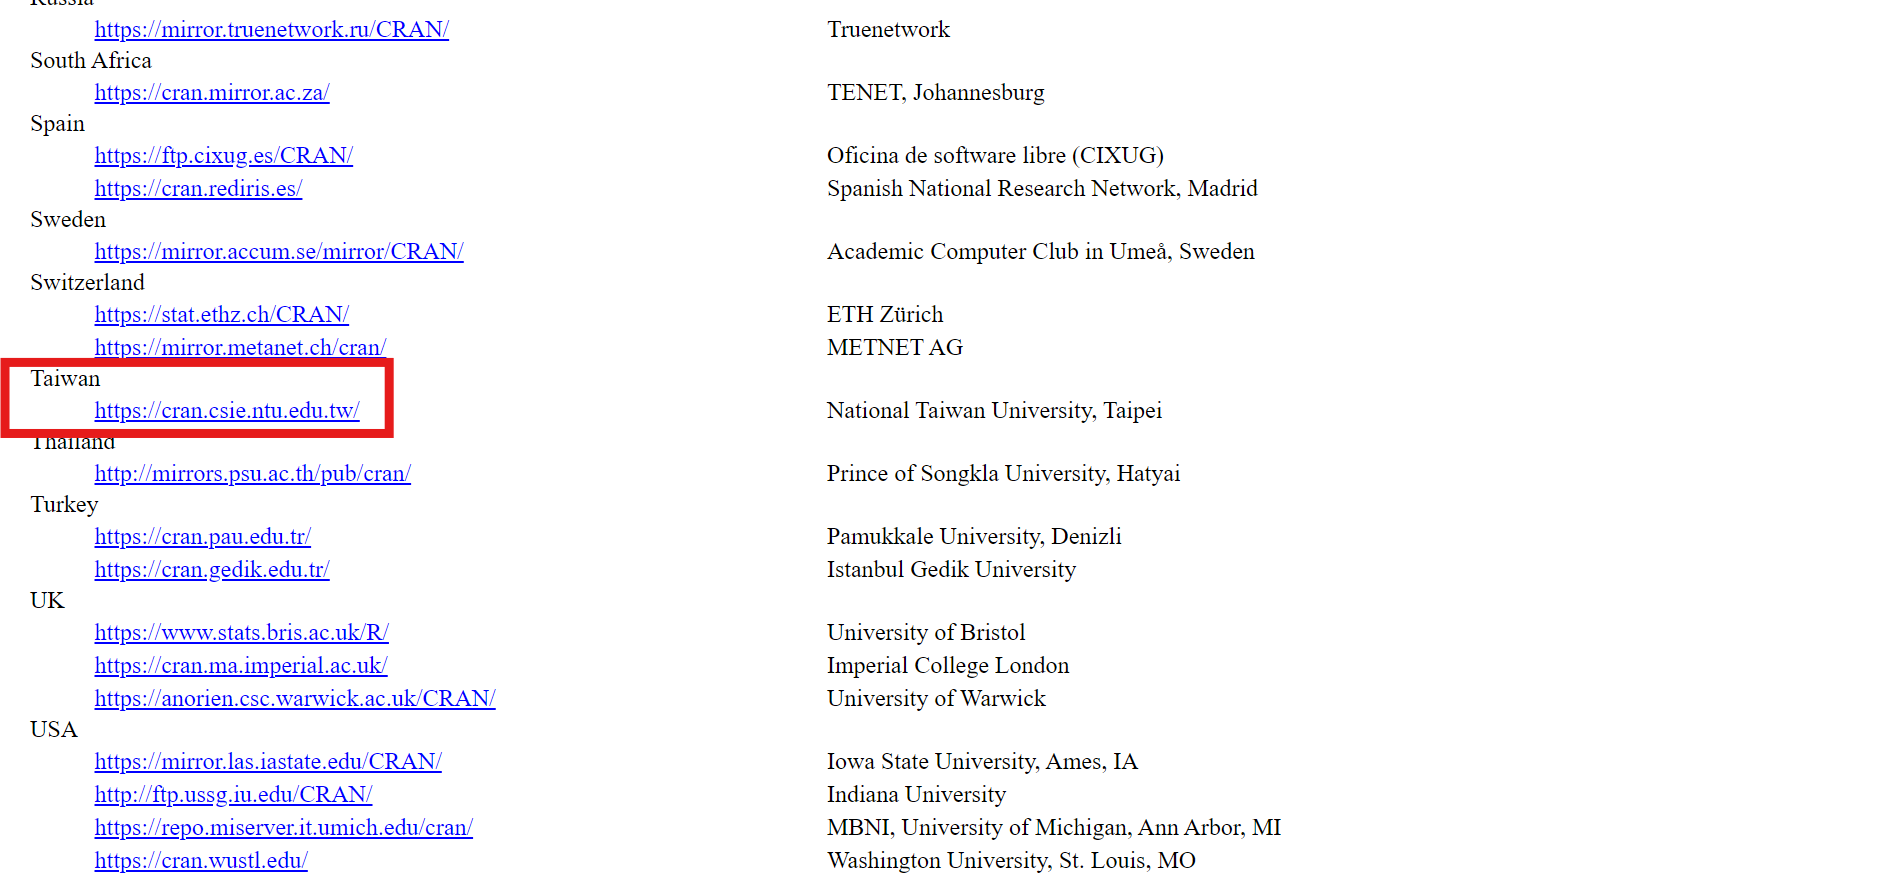
\includegraphics{./assets/images/RWebsite_CRAN.png}

Now you need to choose the files to download according to the system of
your computer. The likeliest to use are for MacOS (if you have a MacBook
computer) or for Windows (if your system is Microsoft).

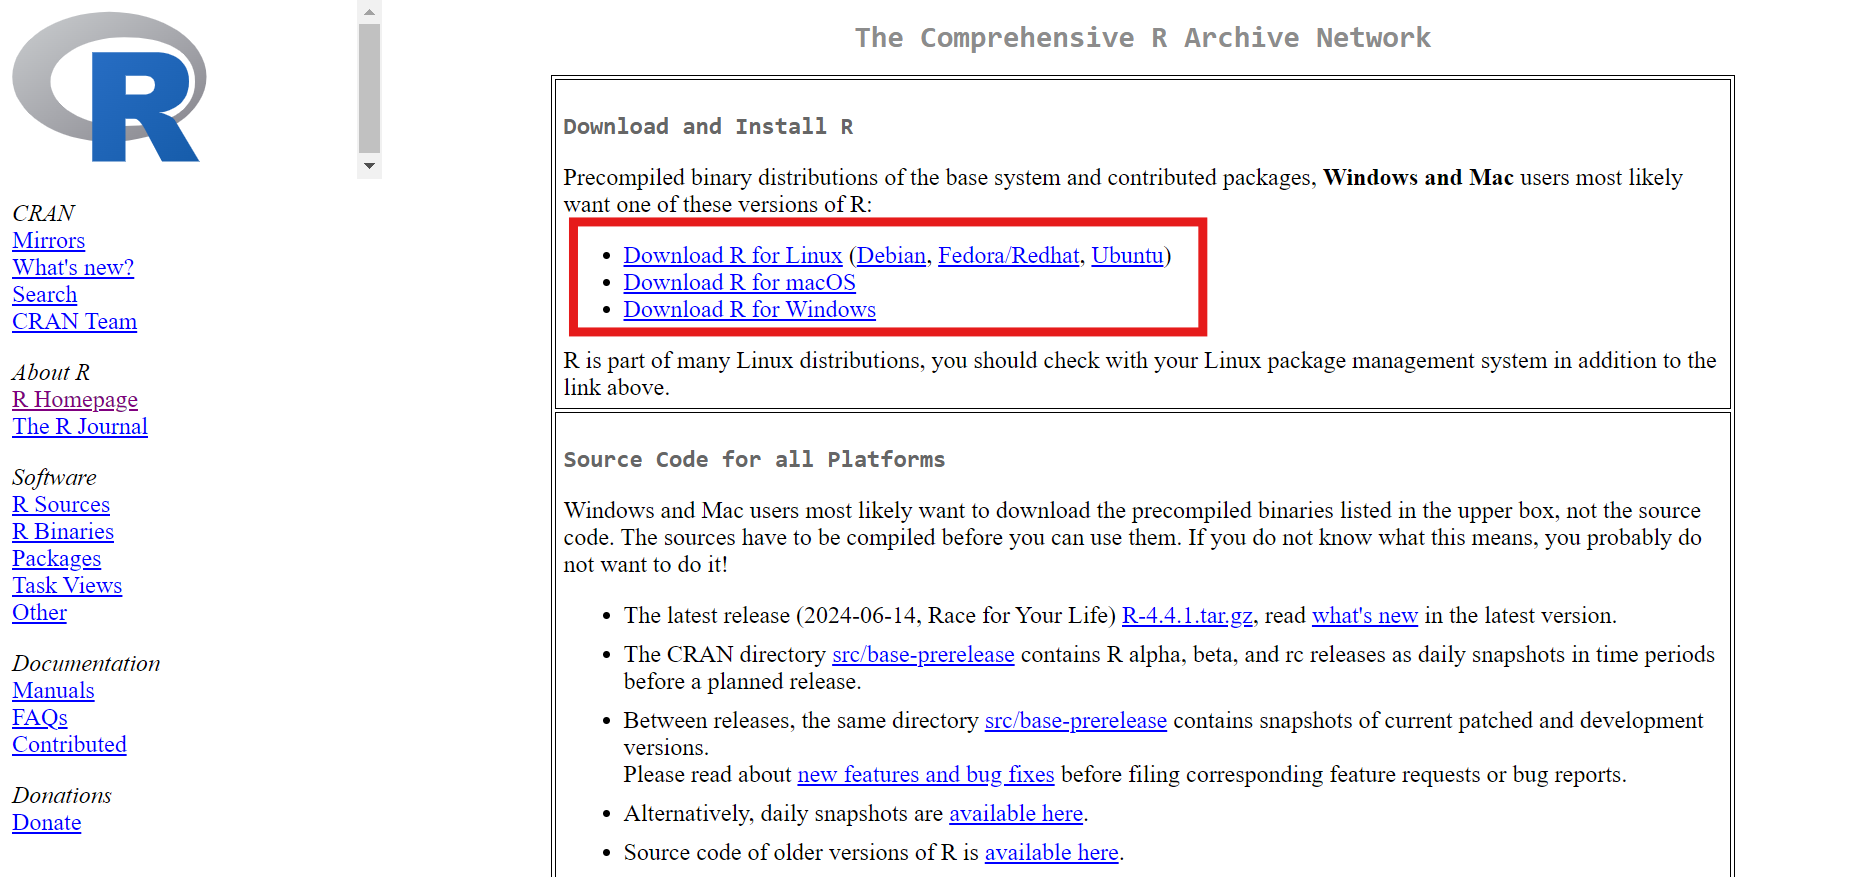
\includegraphics{./assets/images/RWebsite_Download.png}

On the next page, you'll need to choose the subdirectory that you need.
For our purposes, we'll only need the ``base'' subdirectory.

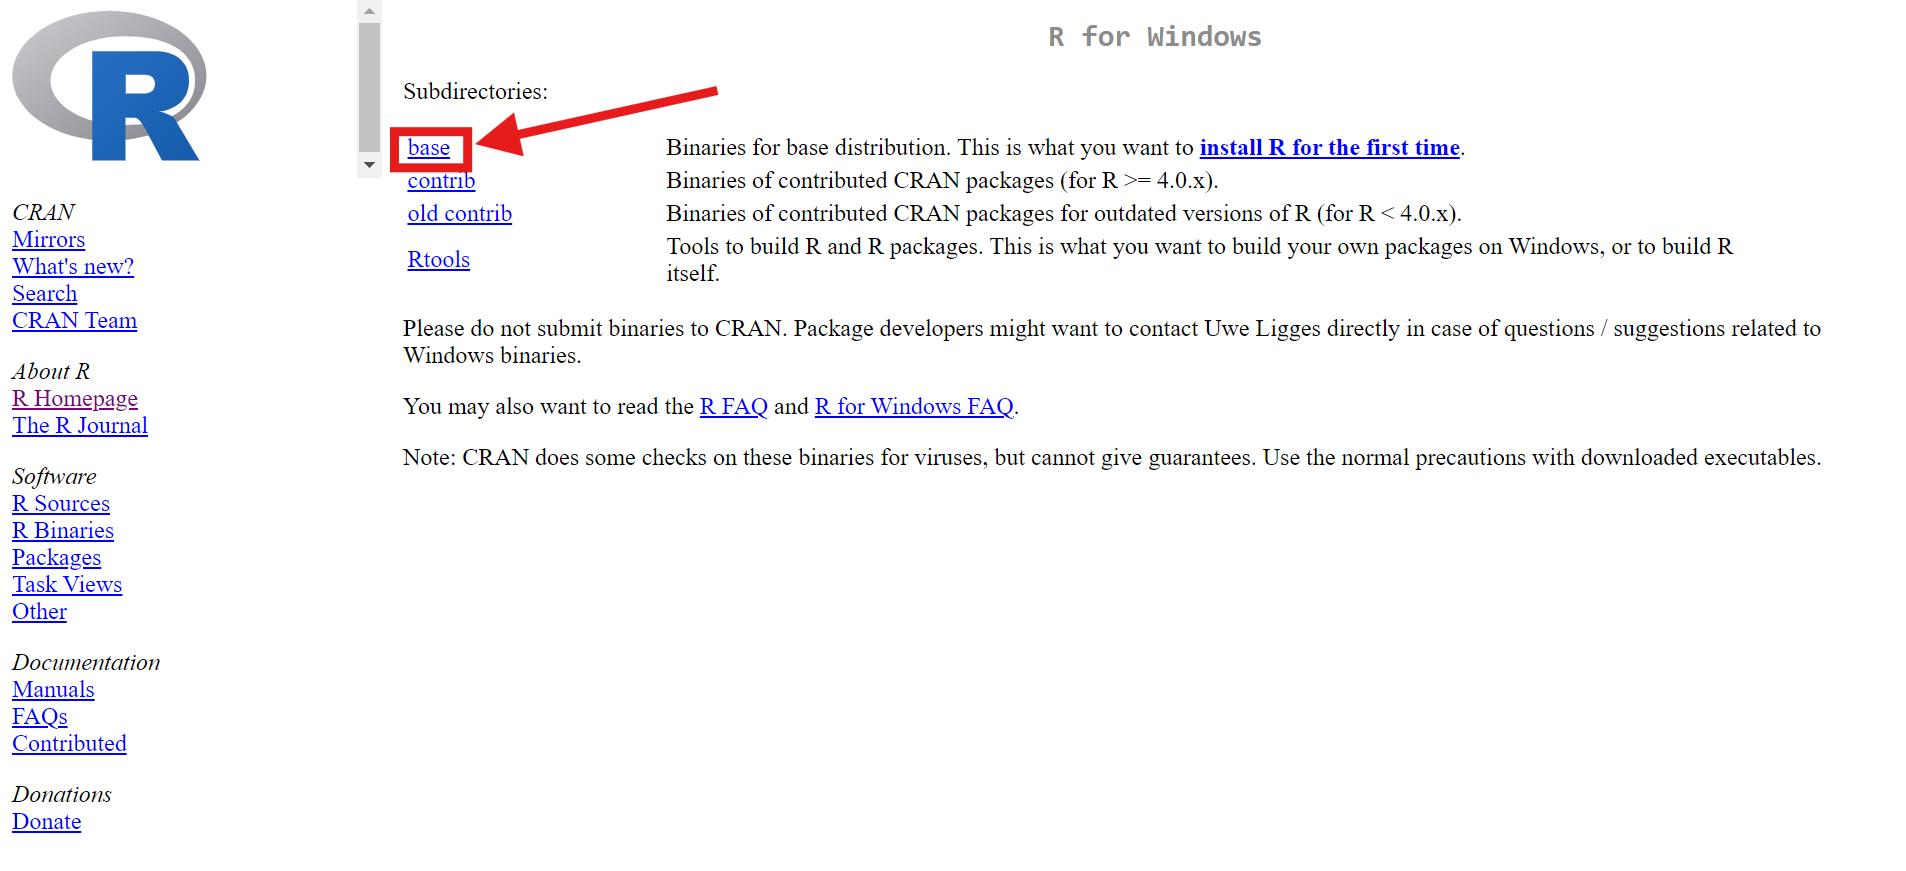
\includegraphics{./assets/images/RWebsite_DownloadSubdirectory.png}

We finally got to the last page! Just click on the first link to
download the files, as in the image below.

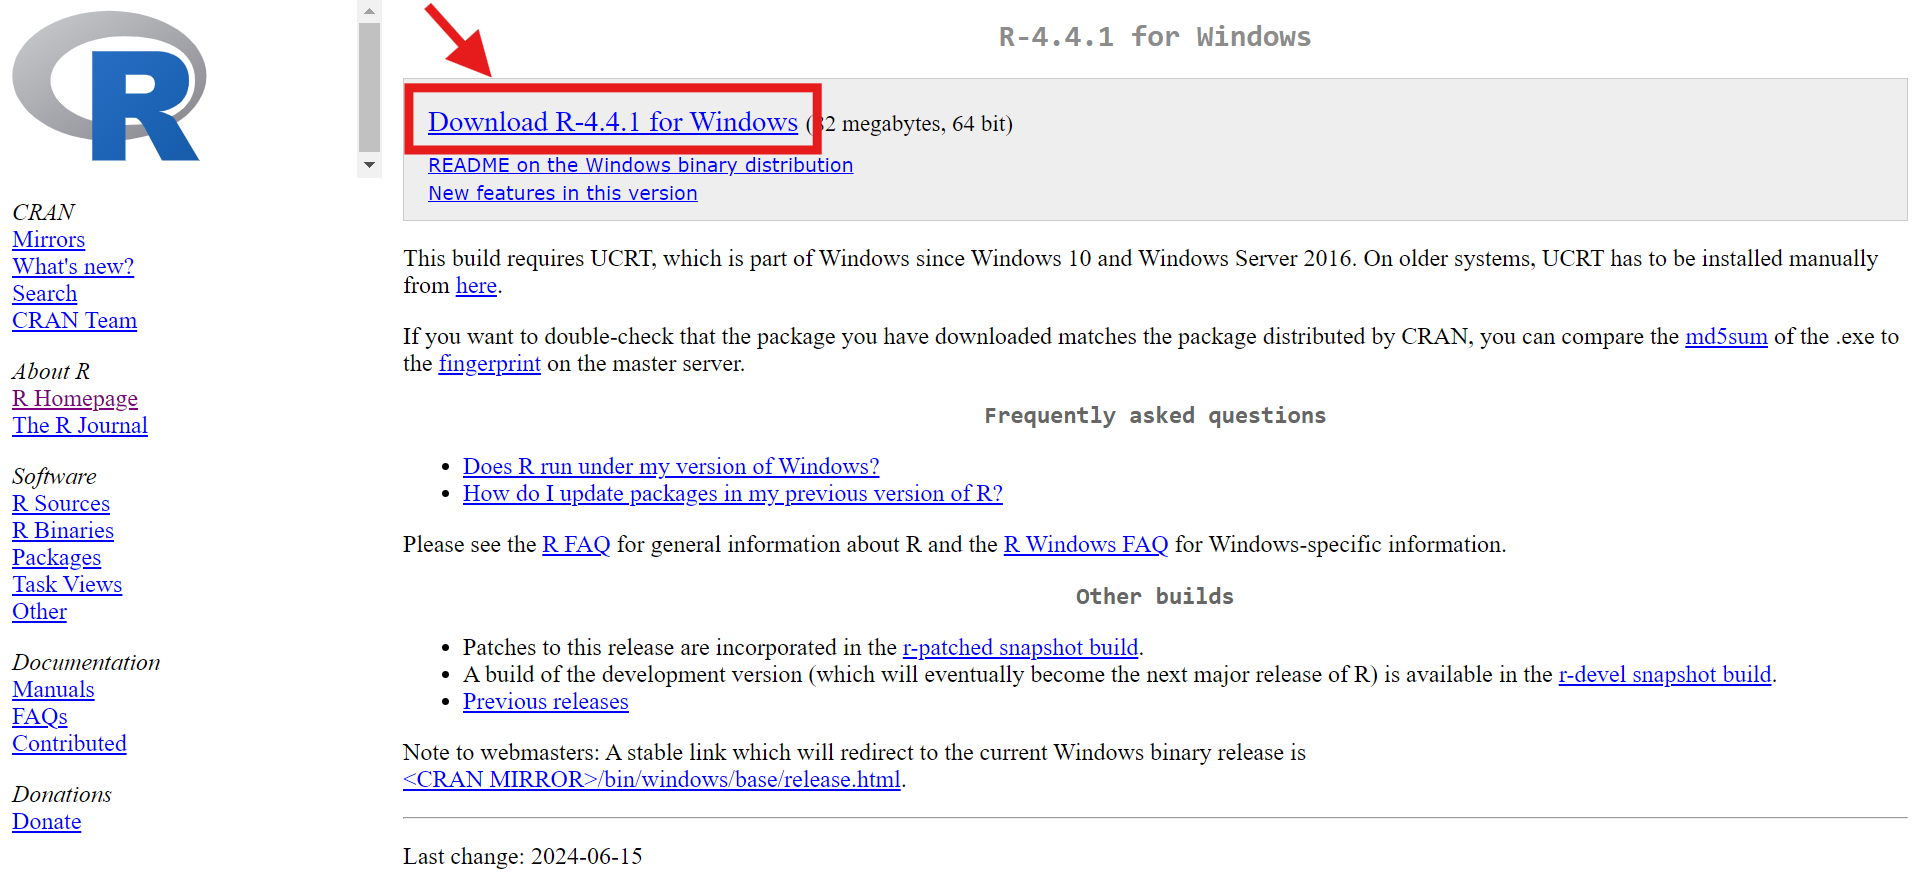
\includegraphics{./assets/images/RWebsite_DownloadFinal.png}

Just wait until the file is downloaded, open it and follow the
instructions to install R on your computer.
\end{block}

\begin{block}{Download and install RStudio}
\protect\hypertarget{download-and-install-rstudio}{}
Now that R is installed on your computer, it is time to do the same with
RStudio. First, let's go to the RStudio website by clicking here , and
you will see something like that (if not, it is just that the RStudio
website has changed):

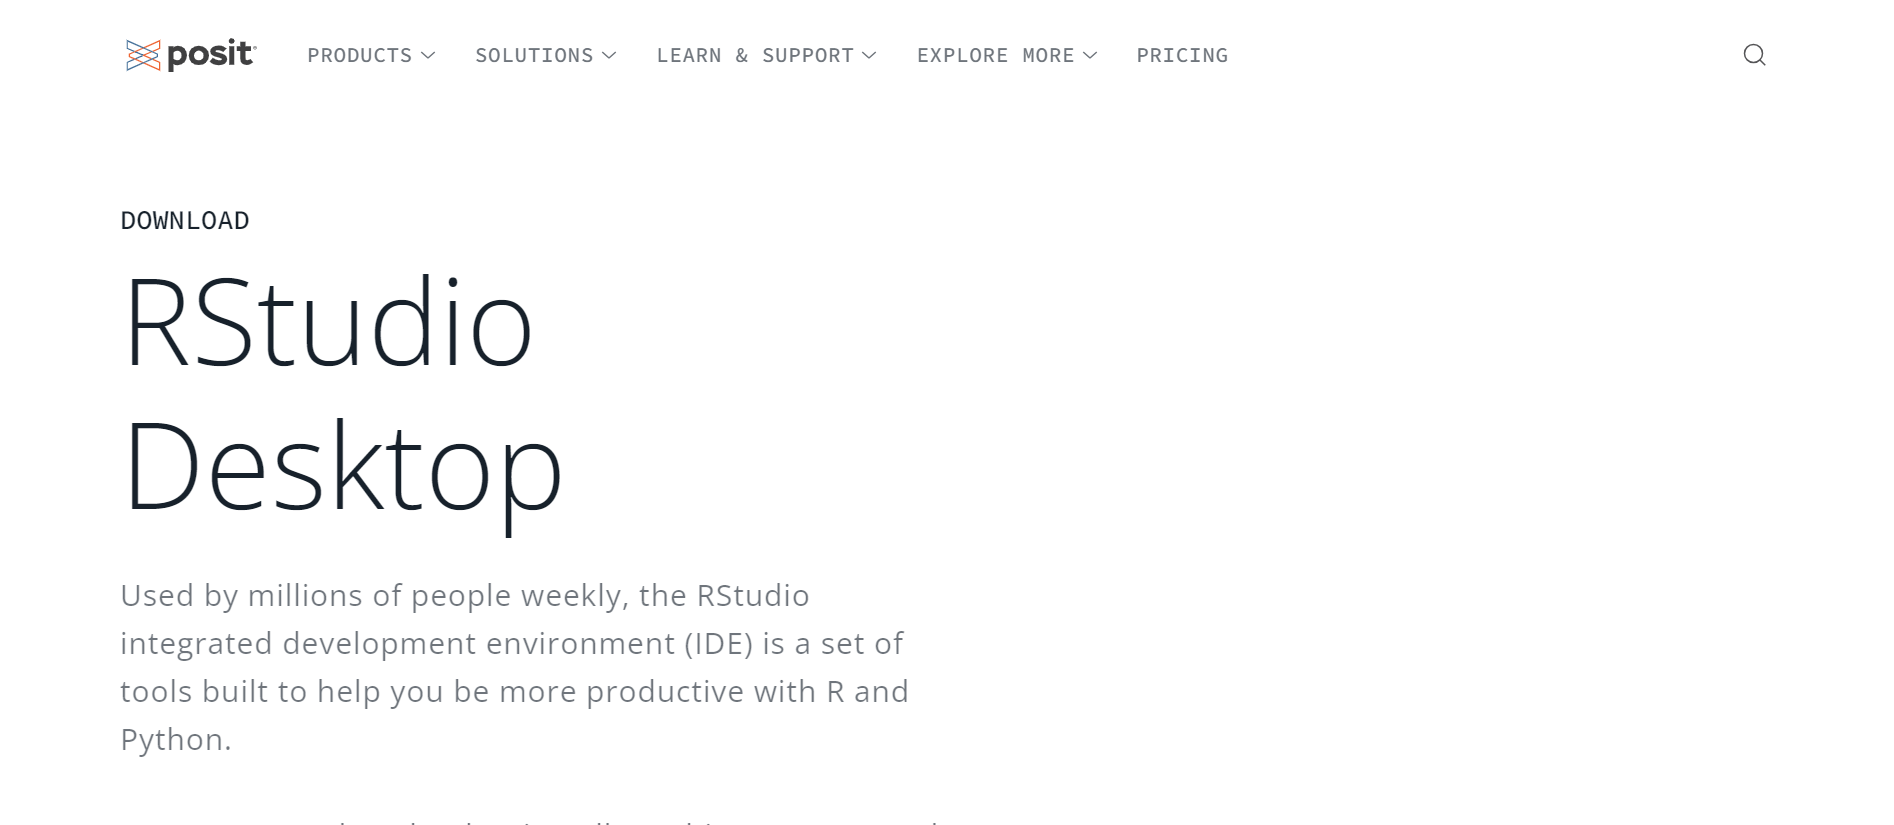
\includegraphics{./assets/images/RStudioWebsite_FrontPage.png}

Once you are on the front page, just scroll down to look for the links
to download the installing files. Again, you will need to choose the
right file to download according to the system of your computer: Window,
macOS (for the most common), or another one.

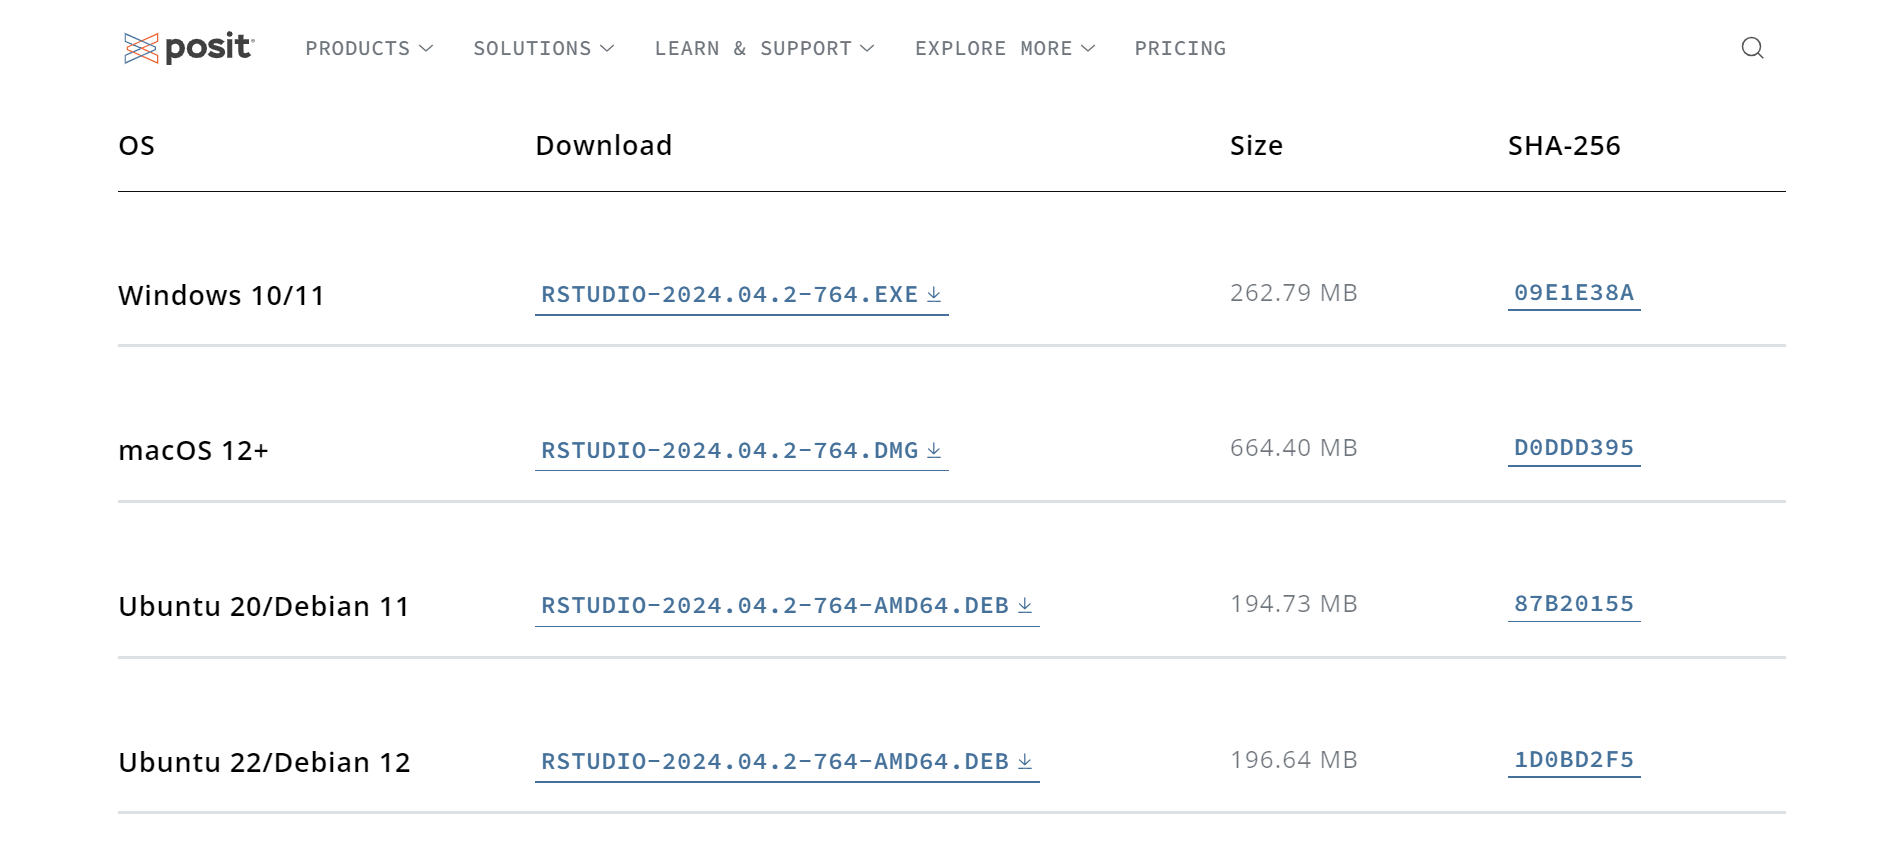
\includegraphics{./assets/images/RStudioWebsite_Download.png}

Just click on the link and the file will start to be downloaded! Again,
give it some minutes, then open the file and follow the instructions to
install RStudio on your computer.
\end{block}
\end{frame}

\begin{frame}{Launch and try!}
\protect\hypertarget{launch-and-try}{}
Look for the program called ``RStudio'' on your computer. Maybe you even
have a shortcut on your desktop after installing it. Once you found it,
just open RStudio, and you can go to the next section!

\begin{tcolorbox}[enhanced jigsaw, colback=white, opacityback=0, bottomrule=.15mm, colframe=quarto-callout-tip-color-frame, rightrule=.15mm, left=2mm, colbacktitle=quarto-callout-tip-color!10!white, leftrule=.75mm, opacitybacktitle=0.6, bottomtitle=1mm, toprule=.15mm, coltitle=black, breakable, toptitle=1mm, titlerule=0mm, title=\textcolor{quarto-callout-tip-color}{\faLightbulb}\hspace{0.5em}{Think about it}, arc=.35mm]

Recall that R is the program where the computations are done, and
RStudio the user-friendly interface. You may ask why I only said to open
the RStudio program when it is only an interface. The good news is, even
if we \emph{need} to download both R and RStudio, you actually only need
to open RStudio when you want to use R!

\end{tcolorbox}
\end{frame}



\end{document}
